\documentclass[]{beamer}
%\documentclass[french,handout]{beamer}

\usepackage{tikz}
\usetikzlibrary{calc}
\usetikzlibrary{positioning}

\usepackage[T1]{fontenc}
\usepackage[utf8]{inputenc}
%\usepackage{mathptmx}
\usepackage[scaled=0.9]{helvet}
\usepackage{tcolorbox}

\usepackage[ruled,lined,longend]{algorithm2e}
\usepackage{tikz}
\usetikzlibrary[topaths]
\usetikzlibrary{arrows.meta,shapes.arrows}


%\usepackage{pgf}
%\usepackage{babel}
\usepackage{eurosym}
\usepackage{mathabx}

\graphicspath{{images/}}

\title[Julia]{Julia tutorial (2)\\ \textbf{Metaheuristic Implementation}}

\date{June 2024}
\author{Prof. Dr. Xavier Gandibleux}\bigskip
\institute{Nantes Université, France} 
%}


\definecolor{colorTD}{rgb}{0.0,0.6,0.7}
\definecolor{colorEL}{rgb}{0.7,0.6,0.0}
\definecolor{BLANC}{rgb}{1.0,1.0,1.0}
\definecolor{ROUGE}{rgb}{1.0,0.0,0.0}
\definecolor{BLEU}{rgb}{0.20,0.22,0.69}
\definecolor{GRIS}{rgb}{0.5,0.5,0.5}
\definecolor{nred}{rgb}{0.8,0.1,0.1}
\definecolor{ngreen}{rgb}{0,0.7,0.4}
\definecolor{nblue}{rgb}{0.2,0.5,0.8}
\definecolor{npink}{rgb}{0.25,0.04,0.87}
\newcommand*{\red}[1]{{\color{nred}#1}}
\newcommand*{\green}[1]{{\color{ngreen}#1}}
\newcommand*{\blue}[1]{\textcolor{nblue}{#1}}
\newcommand*{\pink}[1]{{\color{npink}#1}}
%\colorlet{BLEU}{Blue}
\newcommand{\grisc}[1]{\color{black!20}#1}

\setbeamertemplate{navigation symbols}{} 
\setbeamertemplate{footline}
{ 
\makebox[0.45\textwidth][l] {\hspace{2em} Metaheuristics International Conference 2024}  \hfill 
\includegraphics[height=0.6cm]{logo3ptsJulia.png} \hfill
\makebox[0.45\textwidth][r]{\href{mailto:Xavier Gandibleux@Univ-Nantes.fr}{Xavier Gandibleux@Univ-Nantes.fr} \quad\quad\insertframenumber\hspace{1em}}
\vskip5pt%
}
\setbeamercovered{transparent}

\begin{document}

% 
% ======================================================================================
%

\begin{frame}
  \titlepage
  \vspace{-1cm}
\end{frame}


\setbeamertemplate{footline}
{ 
\makebox[0.45\textwidth][l] {\hspace{2em} Metaheuristics with Julia}  \hfill 
\includegraphics[height=0.4cm]{logo3ptsJulia.png} \hfill
\makebox[0.45\textwidth][r]{\href{mailto:Xavier Gandibleux@Univ-Nantes.fr}{Xavier Gandibleux@Univ-Nantes.fr} \quad\quad\insertframenumber\hspace{1em}}
\vskip4pt%
}


% 
% -------------------------------------------------------------------------------------------------------------------------------------------------------
%
\begin{frame}[fragile]
  \frametitle{Julia}
 \vspace{2mm}

My story with Julia and JuMP: \blue{ROADEF'2016 (Feb 2016)}
 \vspace{6mm}

\centerline{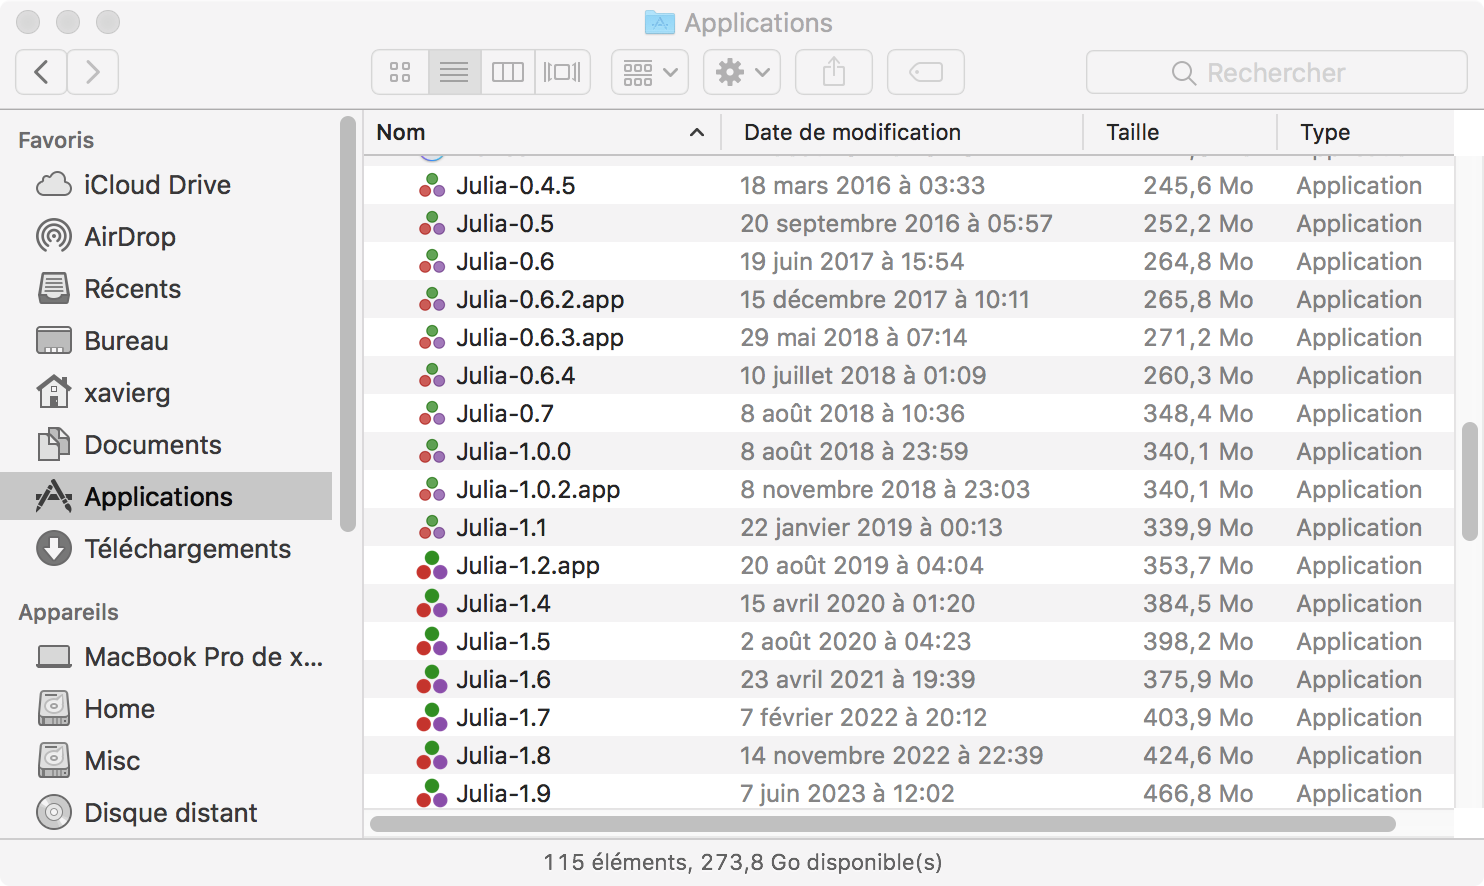
\includegraphics[width=8.5cm]{timelineJulia.png}}

\end{frame}

% 
% -------------------------------------------------------------------------------------------------------------------------------------------------------
%
\begin{frame}[fragile]
  \frametitle{Julia}
 \vspace{2mm}

A programming language for optimization
 \hspace{-5mm}
%  \only<1>{\centerline{\includegraphics[width=12.5cm]{twolanguage1.png}}}
%  \only<2>{\centerline{\includegraphics[width=12.5cm]{twolanguage2.png}}}
%  \only<3>{\centerline{\includegraphics[width=12.5cm]{twolanguage3.png}}}
%  \only<4>
  {\centerline{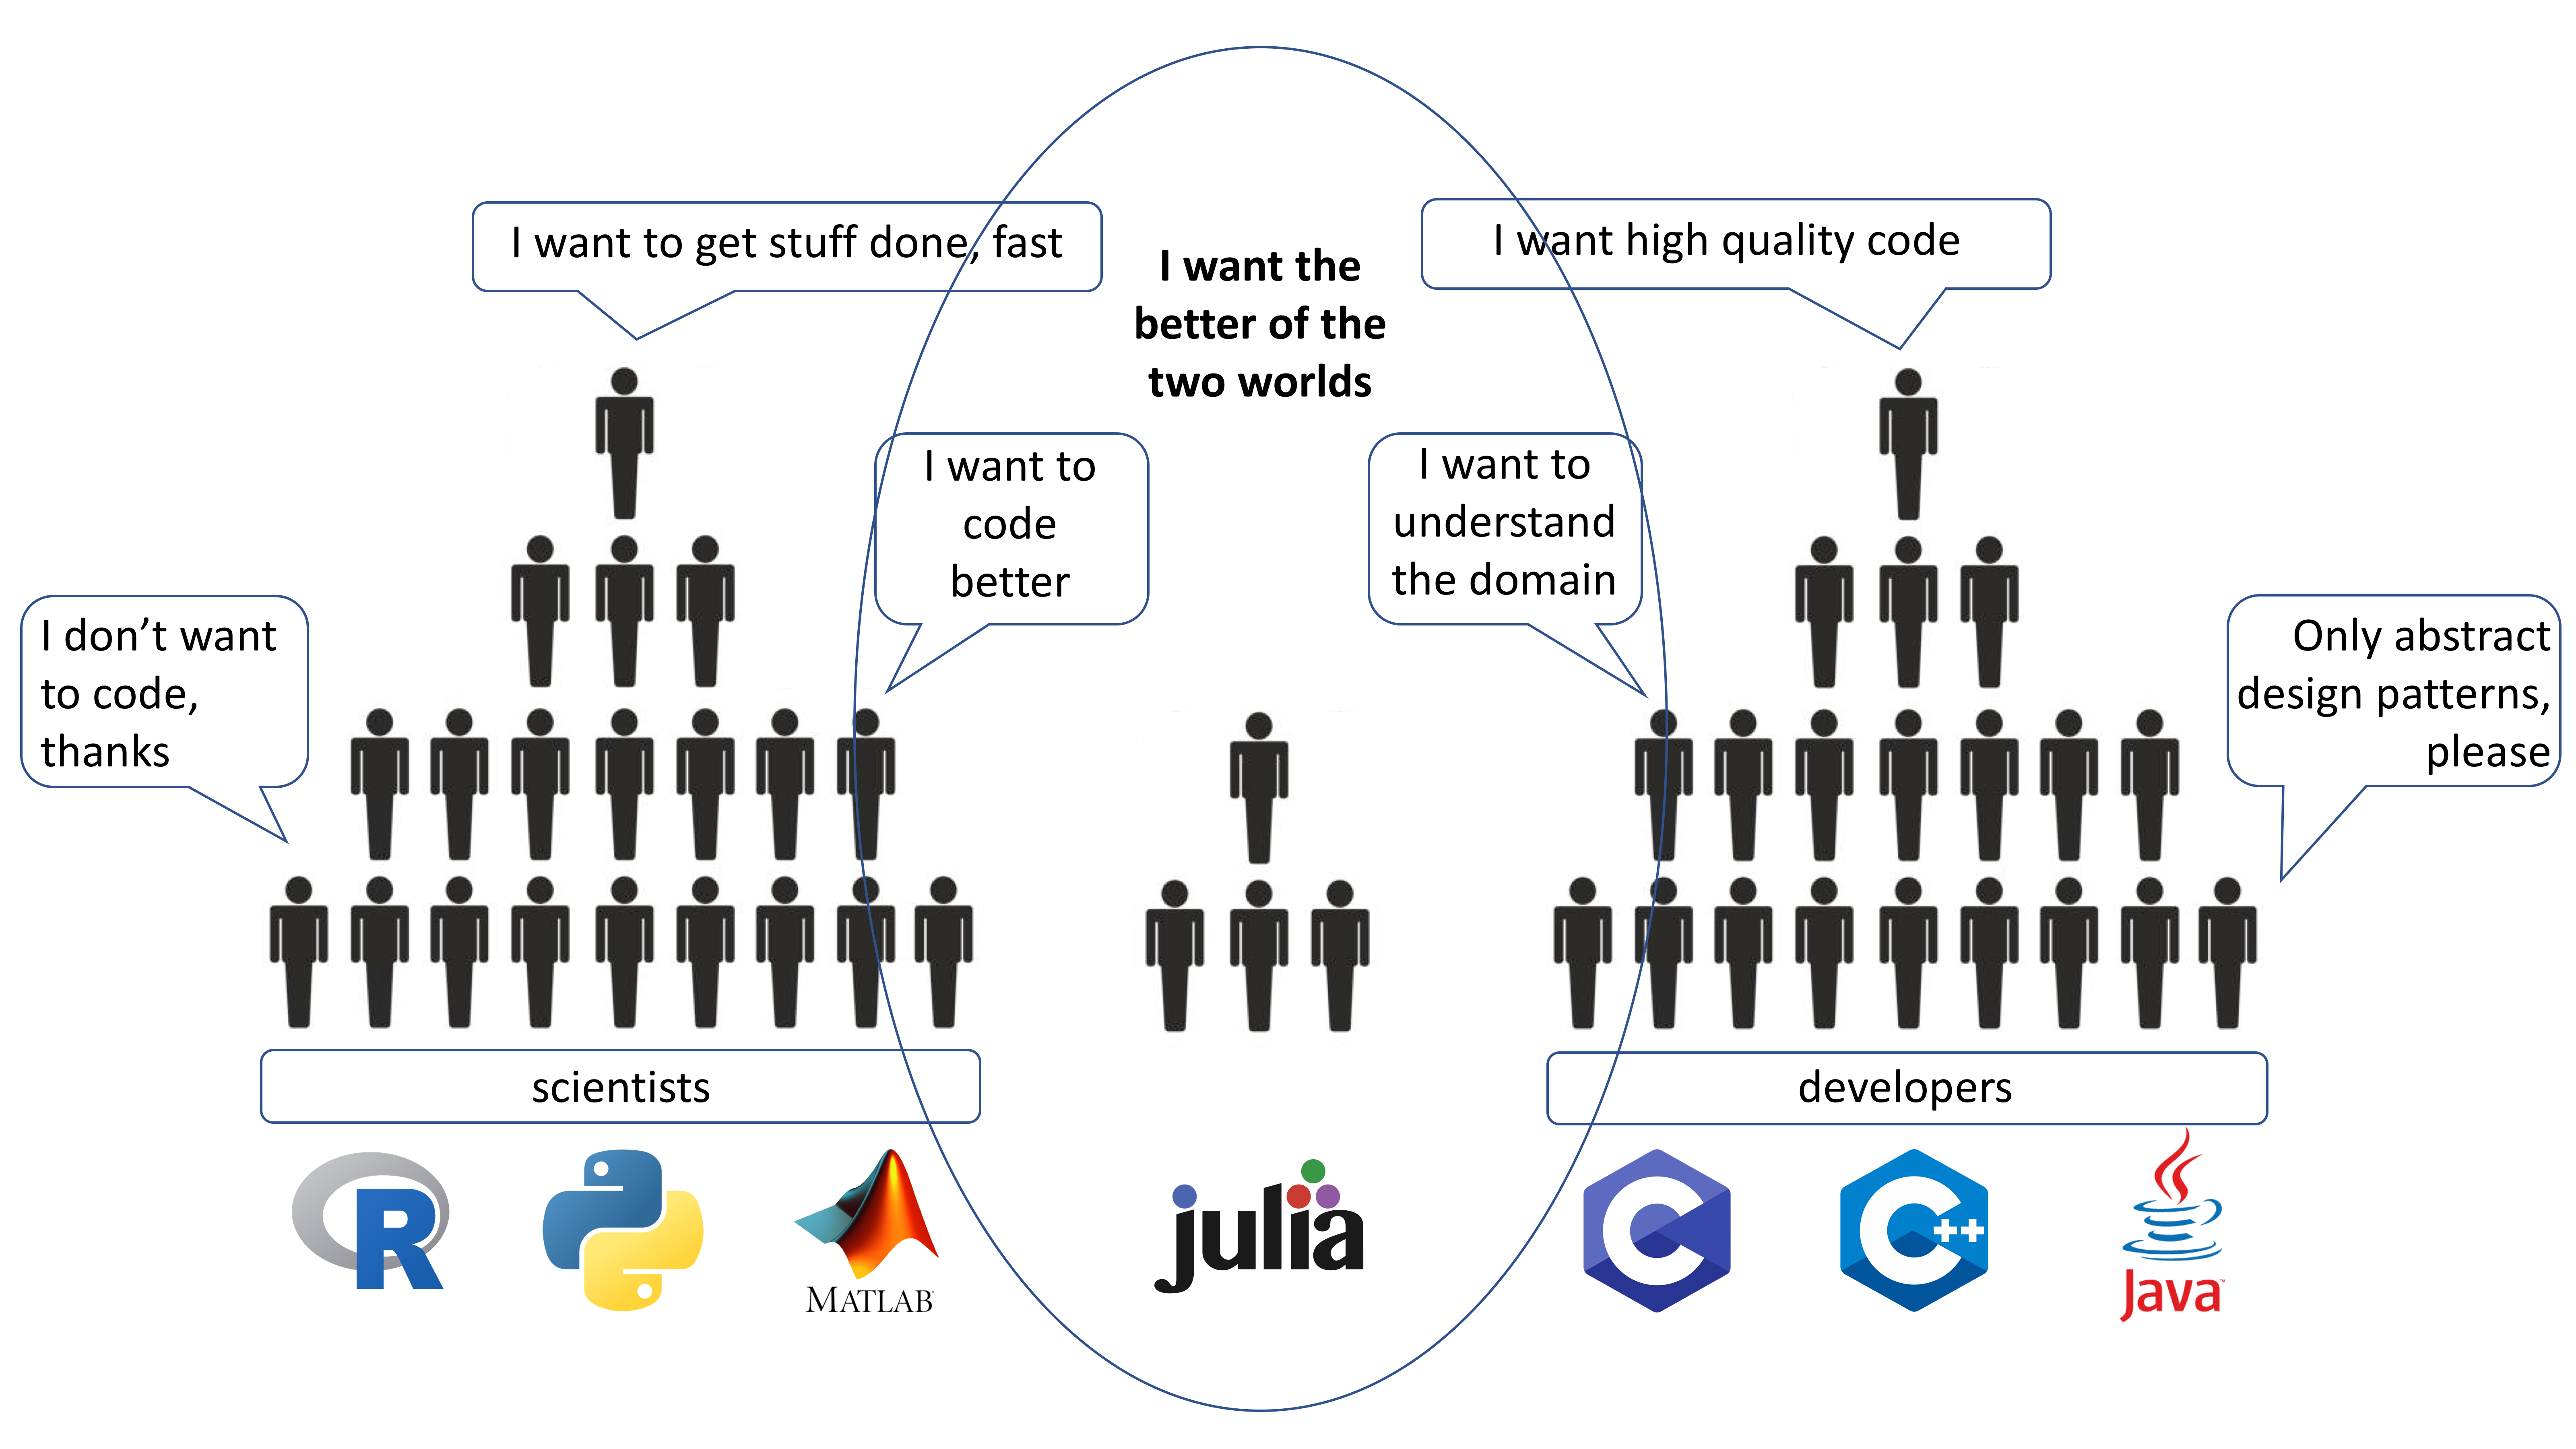
\includegraphics[width=12.5cm]{twolanguage4.png}}}

\end{frame}

% 
% -------------------------------------------------------------------------------------------------------------------------------------------------------
%
\begin{frame}[fragile]
  \frametitle{Julia}
 \vspace{2mm}

LLVM: middleman between source code and compiled native code
 \hspace{-5mm}
  \only<1>{\centerline{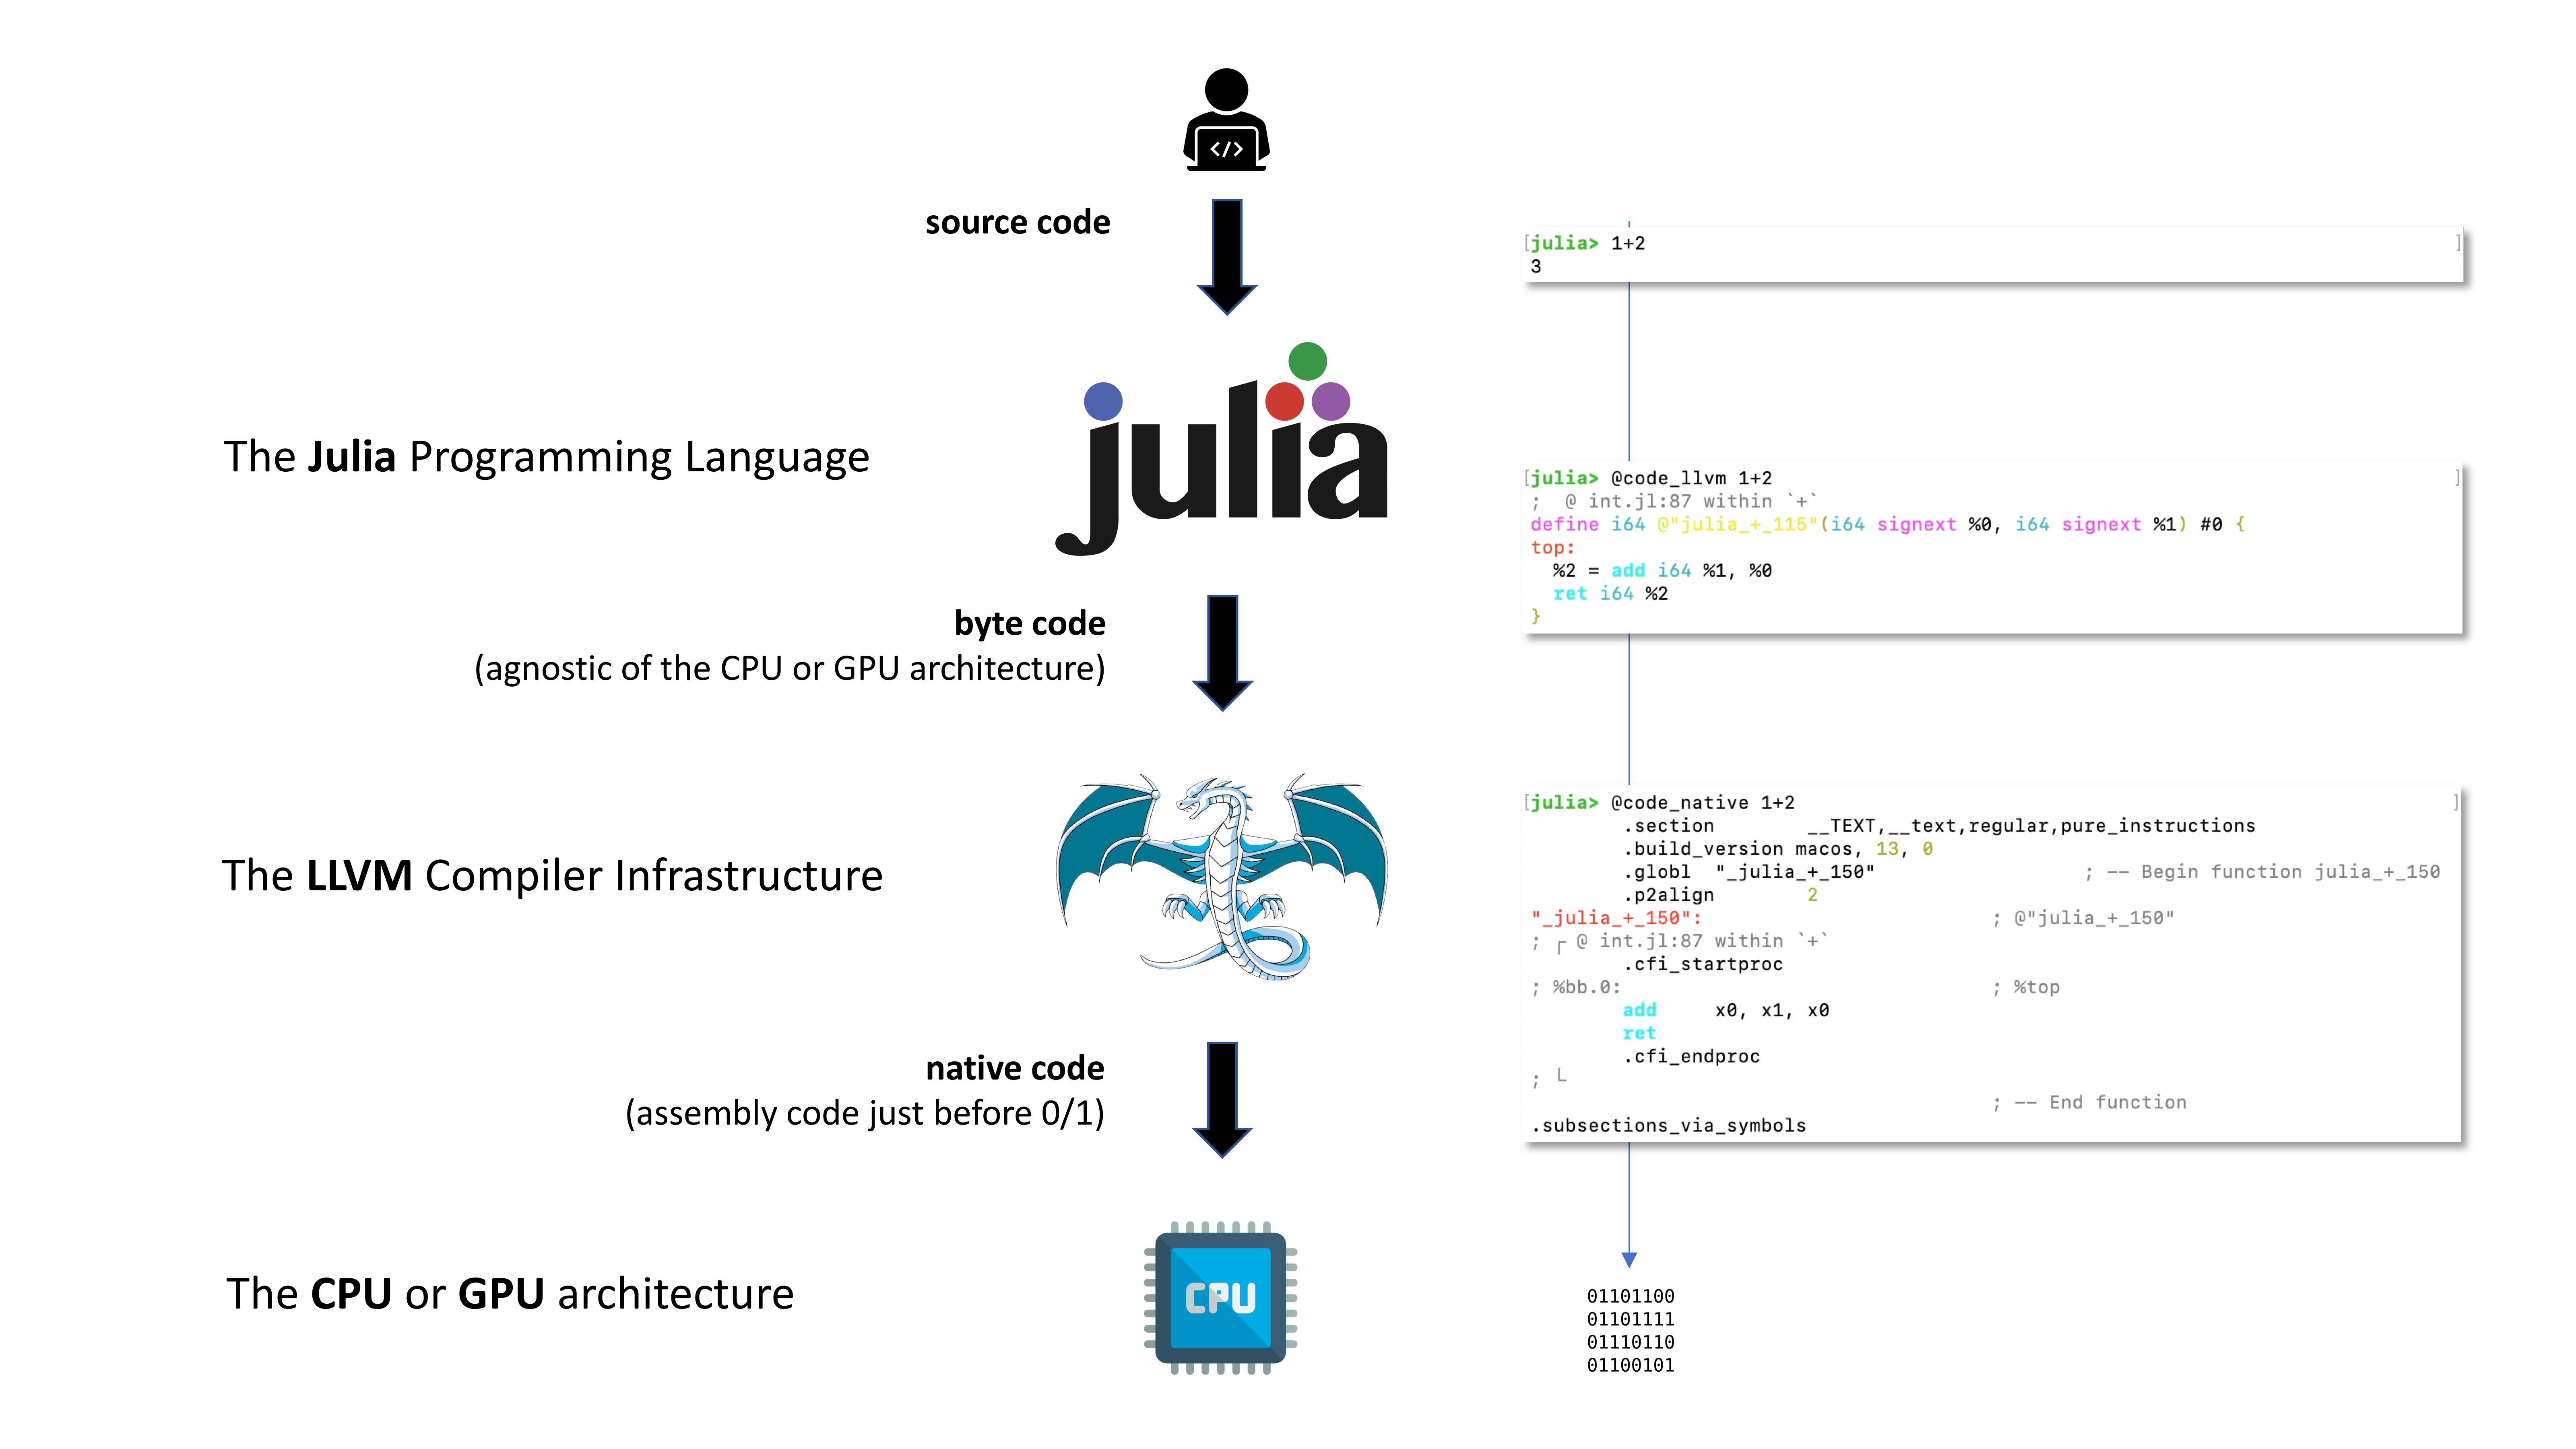
\includegraphics[width=12.5cm]{JuliaLLVM.png}}}
\end{frame}


% 
% -------------------------------------------------------------------------------------------------------------------------------------------------------
%

\begin{frame}
  \frametitle{Problem Support}
\vspace{-4mm}

Set Packing Problem (SPP):
%
\vspace{2ex}
\begin{itemize}
	\item [$\circ$] $J=\{1,\ldots,n\}$ 
	\item [$\circ$] $I=\{1,\ldots,m\}$
	\item [$\circ$] 
\end{itemize}	
%
\vspace{-8mm}

%
\begin{equation*} \label{eqSPP} \renewcommand{\arraystretch}{1.5}
 \quad
  \left[ \begin{array}{r@{}l@{}l}
    Max \ z(x) = & \displaystyle\sum_{j \in J} c_j x_j &\\
    & \displaystyle\sum_{j \in J} a_{i,j} x_j \leq 1 &, \forall i \in I\\
    & x_j \in \{0,1\} &, \forall j \in J\\
    & a_{i,j} \in \{0,1\} &, \forall i \in I, \forall j \in J
  \end{array} \right] \quad (SPP)
\end{equation*}


\end{frame}
%\setbeamertemplate{background canvas}[default]


%
%-----------------------------------------------------------
%

\begin{frame}
  \frametitle{Problem Support}
%\vspace{2mm}

Example of a numerical instance:
\vspace{4mm}

  \begin{columns}
    \begin{column}{.10\textwidth}
    \end{column}
    \begin{column}{.25\textwidth}
   {\footnotesize
    \texttt{7 6                 \\
    7 2 4 6 3 1     \\
    3                    \\
    1 2 3              \\
    3                    \\
    2 5 6              \\
    3                    \\ 
    1 2 4              \\
    3                    \\
    2 3 5              \\
    2                    \\
    4 6                 \\
    3                    \\
    3 4 5              \\
    2                    \\
    1 5                 \\ 
    }
    }
    \end{column}
    \begin{column}{.65\textwidth}
    Format OR-library: {\tiny \url{http://people.brunel.ac.uk/~mastjjb/jeb/info.html}} \\
    \bigskip
    
    number of rows (m), number of columns (n)\\
    \medskip
the cost of each column c(j),j=1,...,n\\
\medskip
for each row i (i=1,...,m): the number of columns which cover row i \\
\medskip
followed by a list of the columns which cover row i
    \end{column}
  \end{columns}
  
\end{frame}


%
%-----------------------------------------------------------
%

\begin{frame}
  \frametitle{Problem Support}
\vspace{-4mm}

Example of a numerical instance:
\vspace{3mm}

{\scriptsize
\begin{center}
$
\left [
\begin{array}{lcrrrrrrrrrrrrllll}
%
   \max z & =  & 7x_1 &+& 2 x_2 &+& 4 x_3 &+&  6 x_4 &+& 3 x_5 &+& x_6 \vspace{2mm}\\	

%  s/c  & &  x_1 &+&  x_2 &+&  x_3  && && && & \ge & 1   \\
%         & &  && x_2 &+& && &&  x_5 &+&  x_6  & \ge & 1   \\
%         & &  x_1 &+&  x_2 &+&  && x_4  && && & \ge & 1  \\
%         & &  && x_2 &+&  x_3 &+&  && x_5 && & \ge & 1  \\
%         & &  && && && x_4 &+& && x_6              & \ge & 1  \\
%         & &  && && x_3 &+&  x_4 &+&  x_5 && & \ge & 1  \\
%         & &  x_1 &+&  && && x_4  && &&            & \ge & 1  \vspace{2mm} \\
%
%  & &  x_1&,& x_2&,& x_3&,& x_4&,& x_5&,& x_6 & = &(0,1)\\
  s/c  & &  x_1 &+&  x_2 &+&  x_3  && && && & \le & 1   \\
         & &  x_2 &+&  x_5 &+&  x_6  & &&&&&&\le & 1   \\
         & &  x_1 &+&  x_2 &+& x_4  && &&&& & \le & 1  \\
         & &  x_2 &+&  x_3 &+&  x_5 && &&&&& \le & 1  \\
         & &  x_4 &+&  x_6 &&&           &&&&  && \le & 1  \\
         & &  x_3 &+&  x_4 &+&  x_5 &&&&&& & \le & 1  \\
         & &  x_1 &+&  x_5  && &&          &&&  && \le & 1  \vspace{2mm} \\

  & &  x_1&,& x_2&,& x_3&,& x_4&,& x_5&,& x_6 & = &(0,1)\\

\end{array}
\right ]
$ 
\end{center}
}

\end{frame}

%
%-----------------------------------------------------------
%

\begin{frame}
  \frametitle{Problem Support}
%\vspace{2mm}

Reading a numerical instance:
\vspace{4mm}

  \begin{columns}
    \begin{column}{.10\textwidth}
    \end{column}
    \begin{column}{.2\textwidth}
   {\footnotesize
    \texttt{7 6                 \\
    7 2 4 6 3 1     \\
    3                    \\
    1 2 3              \\
    3                    \\
    2 5 6              \\
    3                    \\ 
    1 2 4              \\
    3                    \\
    2 3 5              \\
    2                    \\
    4 6                 \\
    3                    \\
    3 4 5              \\
    2                    \\
    1 5                 \\ 
    }
    }
    \end{column}
    \begin{column}{.75\textwidth}
    %
    {\scriptsize
    \begin{tcolorbox}[arc=1ex, colback=black!20, colframe=black!20, left=3pt, right=3pt, top=3pt, bottom=2pt]
    \texttt{ \hspace{-1.5mm}\green{julia>}  function loadSPP(fname)}\\
    \texttt{ \hspace{-1.5mm}\green{julia>}  \hspace{2mm} f = open(fname)}\\
    \texttt{ \hspace{-1.5mm}\green{julia>}  \hspace{2mm} m,n = parse.(Int, split(readline(f)) )}\\
    \texttt{ \hspace{-1.5mm}\green{julia>}  \hspace{2mm} C = parse.(Int, split(readline(f)) )}\\
    \texttt{ \hspace{-1.5mm}\green{julia>}  \hspace{2mm} A = zeros(Int, m, n)}\\
    \texttt{ \hspace{-1.5mm}\green{julia>}  \hspace{2mm} for i=1:m}\\
    \texttt{ \hspace{-1.5mm}\green{julia>}  \hspace{6mm}   readline(f)}\\
    \texttt{ \hspace{-1.5mm}\green{julia>}  \hspace{6mm}   for valeur in split(readline(f))}\\
    \texttt{ \hspace{-1.5mm}\green{julia>}  \hspace{9mm}       j = parse(Int, valeur)}\\
    \texttt{ \hspace{-1.5mm}\green{julia>}  \hspace{9mm}        A[i,j] = 1}\\
    \texttt{ \hspace{-1.5mm}\green{julia>}  \hspace{6mm}      end}\\
    \texttt{ \hspace{-1.5mm}\green{julia>}  \hspace{2mm} end}\\
    \texttt{ \hspace{-1.5mm}\green{julia>}  \hspace{2mm} close(f)}\\
    \texttt{ \hspace{-1.5mm}\green{julia>}  \hspace{2mm} return C, A}\\
    \texttt{ \hspace{-1.5mm}\green{julia>}  end}
    \end{tcolorbox}  
    }
    %
    \end{column}
  \end{columns}
  
\end{frame}




% 
% -------------------------------------------------------------------------------------------------------------------------------------------------------
%

\begin{frame}
  \frametitle{Exercise 0}
\vspace{3mm}

\begin{itemize}
\item \textbf{Solving the SPP instance with a MIP solver}
\smallskip

Modeling the SPP with JuMP, calling your favorite MIP solver
\medskip

%\textcolor{red}{$\rightarrow$ Exact resolution}
\vspace{8mm}

\end{itemize}


\end{frame}

% 
% -------------------------------------------------------------------------------------------------------------------------------------------------------
%

\begin{frame}
  \frametitle{Overview of JuMP}
\vspace{3mm}


%\hspace{-2mm}
A modeling language for Mathematical Optimization (linear, mixed-integer, conic, semidefinite, nonlinear):
\pause

\begin{itemize}
\item \blue{\textbf{User friendliness}}:
syntax that mimics natural mathematical expressions.
\medskip
\pause

\item \blue{\textbf{Speed}}:
similar speeds to special-purpose modeling languages such as AMPL.
\medskip
\pause

\item \blue{\textbf{Solver independence}}:
JuMP uses \textit{MathOptInterface (MOI)},  an abstraction layer designed to provide a unified interface to mathematical optimization solvers. \\
\medskip
Currently supported solvers: Artelys Knitro, Baron, Bonmin, Cbc, Clp, Couenne, CPLEX, FICO Xpress, GLPK, Gurobi, SCIP, etc.
\medskip
\pause

\item \blue{\textbf{Ease of embedding}}:
JuMP itself is written purely in Julia. Solvers are the only binary dependencies.

\end{itemize}

\end{frame}

% 
% -------------------------------------------------------------------------------------------------------------------------------------------------------
%

\begin{frame}
  \frametitle{Getting Started}
\vspace{3mm}

\hspace{-2mm}Install:
\vspace{1mm}
{\scriptsize
\begin{tcolorbox}[arc=1ex, colback=black!20, colframe=black!20, left=3pt, right=3pt, top=3pt, bottom=2pt]
\texttt{ \hspace{-1.5mm}\green{julia>}  using Pkg}
%$\mbox{}$\hspace{0mm}   Pkg.add("JuMP")}
\end{tcolorbox}  
\vspace{1mm}
\pause
\begin{tcolorbox}[arc=1ex, colback=black!20, colframe=black!20, left=3pt, right=3pt, top=3pt, bottom=2pt]
\texttt{ \hspace{-1.5mm}\green{julia>}  Pkg.add("JuMP")}
\end{tcolorbox}  
\vspace{1mm}
\pause
\begin{tcolorbox}[arc=1ex, colback=black!20, colframe=black!20, left=3pt, right=3pt, top=3pt, bottom=2pt]
\texttt{ \hspace{-1.5mm}\green{julia>}   Pkg.add("HiGHS")}
\end{tcolorbox}
\vspace{1mm}
\pause
\begin{tcolorbox}[arc=1ex, colback=black!20, colframe=black!20, left=3pt, right=3pt, top=3pt, bottom=2pt]
\texttt{ \hspace{-1.5mm}\green{julia>}   Pkg.add("Gurobi")}
\end{tcolorbox}
%\pause
\vspace{3mm}
}

%\hspace{-2mm}Setup:
%\vspace{1mm}
%\begin{tcolorbox}[arc=1ex, colback=blue!20, colframe=blue!20, left=3pt, right=3pt, top=3pt, bottom=2pt]
%\texttt{ \hspace{-2mm}  using JuMP}
%\end{tcolorbox}  
%\vspace{-1mm}
%\begin{tcolorbox}[arc=1ex, colback=blue!20, colframe=blue!20, left=3pt, right=3pt, top=3pt, bottom=2pt]
%\texttt{ \hspace{-2mm}  using HiGHS}
%\end{tcolorbox}  
%\vspace{1mm}

\end{frame}

% 
% -------------------------------------------------------------------------------------------------------------------------------------------------------
%

\begin{frame}
  \frametitle{Writing a SPP Model and Solving an Instance}
\vspace{3mm}

{\scriptsize
\begin{tcolorbox}[arc=1ex, colback=black!20, colframe=black!20, left=3pt, right=3pt, top=3pt, bottom=2pt]
\texttt{ \hspace{-1.5mm}\green{julia>}  using JuMP, HiGHS}
\end{tcolorbox} 

\begin{tcolorbox}[arc=1ex, colback=black!20, colframe=black!20, left=3pt, right=3pt, top=3pt, bottom=2pt]
    \texttt{ \hspace{-1.5mm}\green{julia>}  C,A = loadSPP(fname)}\\
    \texttt{ \hspace{-1.5mm}\green{julia>}  m,n = size(A)}   
\end{tcolorbox} 

\begin{tcolorbox}[arc=1ex, colback=black!20, colframe=black!20, left=3pt, right=3pt, top=3pt, bottom=2pt]
%\texttt{ \hspace{-2mm}\green{julia>}  using JuMP, HiGHS}\\
\texttt{ \hspace{-1.5mm}\green{julia>}  spp = Model(HiGHS.Optimizer)}\\
\texttt{ \hspace{-2mm}\green{julia>}  @variable(spp, x[1:n], Bin)}\\
\texttt{ \hspace{-2mm}\green{julia>}  @objective(spp, Max, sum(c[j]*x[j] for j=1:n))} \\
\texttt{ \hspace{-2mm}\green{julia>}  @constraint(spp, cst[i=1:m], sum(A[i,j]*x[j] for j=1:n) $\le$ 1)}
\end{tcolorbox} 

\begin{tcolorbox}[arc=1ex, colback=black!20, colframe=black!20, left=3pt, right=3pt, top=3pt, bottom=2pt]
\texttt{ \hspace{-1.5mm}\green{julia>}   print(model)}
\end{tcolorbox} 

\begin{tcolorbox}[arc=1ex, colback=black!20, colframe=black!20, left=3pt, right=3pt, top=3pt, bottom=2pt]
\texttt{ \hspace{-1.5mm}\green{julia>}  optimize!(model)}
\end{tcolorbox} 

 \begin{tcolorbox}[arc=1ex, colback=black!20, colframe=black!20, left=3pt, right=3pt, top=3pt, bottom=2pt]
  \texttt{ \hspace{-1.5mm}\green{julia>}   @show objective\_value(model)}\\   
    \texttt{ \hspace{-2mm}\green{julia>}  @show  value(x[2])}\\
    \texttt{ \hspace{-2mm}\green{julia>}  @show  value.(x)}    
    \end{tcolorbox} 
    \vspace{3mm}    
}

\end{frame}


% 
% -------------------------------------------------------------------------------------------------------------------------------------------------------
%

\begin{frame}
  \frametitle{Exercise 1}
\vspace{3mm}

\begin{itemize}
\item \textbf{Construct a ``good'' initial solution}
\smallskip

Iterative procedure: selection parts of a solution until it is feasible
\medskip

%\textcolor{red}{$\rightarrow$ Construction algorithm}
\vspace{8mm}

\item \textbf{Improve a ``good'' feasible solution}
\smallskip

Iterative procedure: move from one solution to an other solution as long as required. The solution is the result of a move into a neighborhood structure.
\medskip

%\textcolor{red}{$\rightarrow$  Local search algorithm}
\end{itemize}


\end{frame}



% 
% -------------------------------------------------------------------------------------------------------------------------------------------------------
%

\begin{frame}
  \frametitle{Construction Algorithm}
\vspace{3mm}

\scalebox{1.0}{ 
    \begin{algorithm}[H] 
\begin{tabular}{@{}p{0.5cm}|l}
\multicolumn{2}{l}{$S \leftarrow \emptyset$}\\
\multicolumn{2}{l}{Initialize the candidate set $\cal{C}$, and evaluate the utility $u(e), \forall e \in \cal{C}$}\\
\multicolumn{2}{l}{\textbf{while } ($\cal{C} \neq \emptyset$) \textbf{loop}}\\
& Select the current $Best$ element $e$ from $\cal{C}$:\\
&$\qquad e \leftarrow$ $\max_{e \in \cal{C}}{u(e)}$\\
& Incorporate $e$ into the solution:\\
&$\qquad S \leftarrow  S \cup  \{e\}$\\ 
&Update the candidate set $\cal{C}$ and reevaluate the utility $u(e), \forall e \in \cal{C}$\\
&$\qquad  \mathcal{C} \leftarrow \mathcal{C}  \setminus  \texttt{conflict}(\{e\}) $\\
\multicolumn{2}{l}{\textbf{endWhile}}\\
\multicolumn{2}{l}{\textbf{return} $S$}
\end{tabular}
\caption{Greedy construction}
\label{algo:GREEDYconstruction}
\end{algorithm}
}

\end{frame}


%
%-----------------------------------------------------------
%

\begin{frame}
  \frametitle{Example: construction (1/1)}
\vspace{3mm}

{\small

$
\begin{array}{r cccccccl}
%
j =   & 1 & 2 & 3 & 4 & 5 & 6 \vspace{1mm}\\	
c_j =   & 7 & 2 & 4 &  6 & 3 & 1 \vspace{1mm}\\	
x_j =   & . & . & . &  . & . & . \vspace{1mm}\\	
  & 1 & 1 & 1 &  0 & 0 & 0  \\
  & 0 & 1 & 0 &  0 & 1 & 1  \\  
  & 1 & 1 & 0 &  1 & 0 & 0  \\ 
a_{ij} =  & 0 & 1 & 1 &  0 & 1 & 0  \\ 
  & 0 & 0 & 0 &  1 & 0 & 1  \\ 
  & 0 & 0 & 1 &  1 & 1 & 0  \\       
  & 1 & 0 & 0 &  0 & 1 & 0  \\
  \\
   \onslide<2->{
\qquad \sum_{i\in I} a_{ij} = &	3 &	4 &	3 &	3 &	4 &	2 \\	
u(x_j) = &	2,3 & 0,5 &  1,3 & 2 &  0,75 & 0,5 \\	
               & \times &  &  &  &  &  & \onslide<2>{ \rightarrow & j^{*} =   1} \vspace{1mm} \\  
\quad & \qquad & \qquad & \qquad & \qquad & \qquad & \qquad & \\
\\ %\qquad {x_{j} :} &	 0 &  1   &   0    &  1    &   1    &   1   &	 & z(x) = 12 \\               
}
\end{array}
$ 
}

\end{frame}

%
%-----------------------------------------------------------
%

\begin{frame}
  \frametitle{Example: construction (1/1)}
\vspace{3mm}

{\small

$
\begin{array}{r cccccccl}
%
j =   & 1 & 2 & 3 & 4 & 5 & 6 \vspace{1mm}\\
c_j =   & 7 & 2 & 4 &  6 & 3 & 1 \vspace{1mm}\\	
x_j =   & 1 & . & . &  . & . & . \vspace{1mm}\\	
  & {\grisc 1} & {\grisc 1} & {\grisc 1} &  {\grisc 0} & {\grisc 0} & {\grisc 0}  \\
  & {0} & { 1} & { 0} &  { 0} & { 1} & { 1}  \\  
  & {\grisc 1} & {\grisc 1} & {\grisc 0} &  {\grisc 1} & {\grisc 0} & {\grisc 0}  \\ 
a_{ij} =  & { 0} & { 1} & { 1} &  { 0} & { 1} & { 0}  \\ 
  & 0 & 0 & 0 &  1 & 0 & 1  \\ 
  & 0 & 0 & 1 &  1 & 1 & 0  \\       
  &  {\grisc 1}  & {\grisc 0} & {\grisc 0} &   {\grisc 0}  & {\grisc 1} & {\grisc 0}  \\
  \\
%   \onslide<2->{
\qquad \sum_{i\in I} a_{ij} = &	3 &	4 &	3 &	3 &	4 &	2 \\	
u(x_j) = &	2,3 & 0,5 &  1,3 & 2 &  0,75 & 0,5 \\	
               & \times &  &  &  &  &  &  \rightarrow & j^{*} =   1 \vspace{1mm} \\  
\quad & \qquad & \qquad & \qquad & \qquad & \qquad & \qquad & \\
\\ %\qquad {x_{j} :} &	 0 &  1   &   0    &  1    &   1    &   1   &	 & z(x) = 12 \\               
%}
\end{array}
$ 
}
 

\end{frame}

%
%-----------------------------------------------------------
%

\begin{frame}
  \frametitle{Example: construction (1/1)}
\vspace{3mm}

{\small

$
\begin{array}{r cccccccl}
%
j =   & 1 & 2 & 3 & 4 & 5 & 6 \vspace{1mm}\\
c_j =   & 7 & 2 & 4 &  6 & 3 & 1 \vspace{1mm}\\	
x_j =   & 1 & 0 & 0 & 0 & 0 & . \vspace{1mm}\\	
  & {\grisc 1} & {\grisc 1} & {\grisc 1} &  {\grisc 0} & {\grisc 0} & {\grisc 0}  \\
  & {0} & { 1} & { 0} &  { 0} & { 1} & { 1}  \\  
  & {\grisc 1} & {\grisc 1} & {\grisc 0} &  {\grisc 1} & {\grisc 0} & {\grisc 0}  \\ 
a_{ij} =  & { 0} & { 1} & { 1} &  { 0} & { 1} & { 0}  \\ 
  & 0 & 0 & 0 &  1 & 0 & 1  \\ 
  & 0 & 0 & 1 &  1 & 1 & 0  \\       
  &  {\grisc 1}  & {\grisc 0} & {\grisc 0} &   {\grisc 0}  & {\grisc 1} & {\grisc 0}  \\
  \\
%   \onslide<2->{
\qquad \sum_{i\in I} a_{ij} = &	3 &	4 &	3 &	3 &	4 &	2 \\	
u(x_j) = &	2,3 & 0,5 &  1,3 & 2 &  0,75 & 0,5 \\	
               & \times &  &  &  &  &  &  \rightarrow & j^{*} =   1 \vspace{1mm} \\  
\quad & \qquad & \qquad & \qquad & \qquad & \qquad & \qquad & \\
\\ %\qquad {x_{j} :} &	 0 &  1   &   0    &  1    &   1    &   1   &	 & z(x) = 12 \\               
%}
\end{array}
$ 
}
 

\end{frame}

%
%-----------------------------------------------------------
%

\begin{frame}
  \frametitle{Example: construction (2/2)}
\vspace{3mm}

{\small

$
\begin{array}{r cccccccl}
%
j =   & 1 & 2 & 3 & 4 & 5 & 6 \vspace{1mm}\\
c_j =   & 7 & 2 & 4 &  6 & 3 & 1 \vspace{1mm}\\	
x_j =   & 1 & 0 & 0 & 0 & 0 & . \vspace{1mm}\\	
  & {\grisc 1} & {\grisc 1} & {\grisc 1} &  {\grisc 0} & {\grisc 0} & {\grisc 0}  \\
  & {0} & { 1} & { 0} &  { 0} & { 1} & { 1}  \\  
  & {\grisc 1} & {\grisc 1} & {\grisc 0} &  {\grisc 1} & {\grisc 0} & {\grisc 0}  \\ 
a_{ij} =  & { 0} & { 1} & { 1} &  { 0} & { 1} & { 0}  \\ 
  & 0 & 0 & 0 &  1 & 0 & 1  \\ 
  & 0 & 0 & 1 &  1 & 1 & 0  \\       
  &  {\grisc 1}  & {\grisc 0} & {\grisc 0} &   {\grisc 0}  & {\grisc 1} & {\grisc 0}  \\
  \\
%   \onslide<2->{
\qquad \sum_{i\in I} a_{ij} = &	- &	- &	- &	- &	- &	2 \\	
u(x_j) = &	- & - &  - & - &  - & 0,5 \\	
               &  &  &  &  &  &  \times &  \rightarrow & j^{*} =   6 \vspace{1mm} \\  
\quad & \qquad & \qquad & \qquad & \qquad & \qquad & \qquad & \\
\\ %\qquad {x_{j} :} &	 0 &  1   &   0    &  1    &   1    &   1   &	 & z(x) = 12 \\               
%}
\end{array}
$ 
}
 

\end{frame}

%
%-----------------------------------------------------------
%

\begin{frame}
  \frametitle{Example: construction (2/2)}
\vspace{3mm}

{\small

$
\begin{array}{r cccccccl}
%
j =   & 1 & 2 & 3 & 4 & 5 & 6 \vspace{1mm}\\
c_j =   & 7 & 2 & 4 &  6 & 3 & 1 \vspace{1mm}\\	
x_j =   & 1 & 0 & 0 & 0 & 0 & 1 \vspace{1mm}\\	
  & {\grisc 1} & {\grisc 1} & {\grisc 1} &  {\grisc 0} & {\grisc 0} & {\grisc 0}  \\
  & {\grisc 0} & {\grisc 1} & {\grisc 0} &  {\grisc 0} & {\grisc 1} & {\grisc 1}  \\  
  & {\grisc 1} & {\grisc 1} & {\grisc 0} &  {\grisc 1} & {\grisc 0} & {\grisc 0}  \\ 
a_{ij} =  & { 0} & { 1} & { 1} &  { 0} & { 1} & { 0}  \\ 
  & {\grisc 0} & {\grisc 0} & {\grisc 0} &  {\grisc 1} & {\grisc 0} & {\grisc 1}  \\ 
  & 0 & 0 & 1 &  1 & 1 & 0  \\       
  &  {\grisc 1}  & {\grisc 0} & {\grisc 0} &   {\grisc 0}  & {\grisc 1} & {\grisc 0}  \\
  \\
%   \onslide<2->{
\qquad \sum_{i\in I} a_{ij} = &	- &	- &	- &	- &	- &	2 \\	
u(x_j) = &	- & - &  - & - &  - & 0,5 \\	
               &  &  &  &  &  &  \times &  \rightarrow & j^{*} =   6 \vspace{1mm} \\  
\quad & \qquad & \qquad & \qquad & \qquad & \qquad & \qquad & \\
\\ %\qquad {x_{j} :} &	 0 &  1   &   0    &  1    &   1    &   1   &	 & z(x) = 12 \\               
%}
\end{array}
$ 
}
 

\end{frame}





% 
% -------------------------------------------------------------------------------------------------------------------------------------------------------
%

\begin{frame}
  \frametitle{Improvement Algorithm (Deepest Descent Method)}
\vspace{3mm}

\scalebox{1.0}{                        %new code
    \begin{algorithm}[H] 
\begin{tabular}{@{}p{0.5cm}|l}
\multicolumn{2}{l}{$S$, a feasible solution}\\
\multicolumn{2}{l}{localOptimum $\leftarrow$ false}\\
\multicolumn{2}{l}{\textbf{repeat } }\\
& Choose $S'  \in \cal{N}(S)$ with $f(S') < f(S)$ \\
& \textbf{if } found($S'$)\\
&  \quad $S \leftarrow S'$\\
& \textbf{else } \\
&  \quad localOptimum $\leftarrow$ true\\
& \textbf{endIf } \\
\multicolumn{2}{l}{\textbf{until } localOptimum }\\
\multicolumn{2}{l}{\textbf{return} $S$}\\
\end{tabular}
\caption{Local search algorithm (for minimization)}
\label{algo:GRASPimprovement}
\end{algorithm}
}

\end{frame}





%
%-----------------------------------------------------------
%

\begin{frame}
  \frametitle{Example: improvement (1/2)}
\vspace{3mm}

A solution $x$ ($x_j =(0,1), \ j=1,\dots,n$) :
\medskip
 
\begin{itemize}
%  \item \redtxt{$add(i)$} : \\
%  	$i\in \{1,..., n\} \ \mid \ x_{i} \nearrow 1$
%	\medskip
%	
%  \item \redtxt{$drop(i)$} : \\
%  	$i\in \{1,..., n\} \ \mid \ x_{i} \searrow 0$
%	\medskip
%	
%  \item \redtxt{$addDrop(i,j)$} : \\
%  	$i,j\in \{1,..., n\} \ \mid \ x_{i} \nearrow 1, \ x_{j} \searrow 0$
%	\medskip
%		
  \item move: \\ 
        \textcolor{red}{$kp$$-exchange$} :\\
  	$k$ variables at 1 switched to 0 and $p$ variables at 0 switched to 1
	\medskip
	
  \item relevant values of $kp$ for WSPP: 	\\
  0-1-exchange\\
  1-1-exchange\\
  1-2-exchange\\
  2-1-exchange\\
  etc.
\end{itemize}

\end{frame}

%
%-----------------------------------------------------------
%

\begin{frame}
  \frametitle{Example: improvement (2/2)}
\vspace{3mm}

1-1-exchange:
\bigskip

{\small

$
\begin{array}{r cccccccl}
%
j =   & 1 & 2 & 3 & 4 & 5 & 6 \vspace{1mm}\\
c_j =   & 7 & 2 & 4 &  6 & 3 & 1 \vspace{1mm}\\	
x_j =   & \quad {\blue 1}\searrow & 0 & \quad {\red 0}\nearrow & 0 & 0 & 1 & \rightarrow z(x)= 8 \vspace{3mm}\\	
  & {\blue 1} & { 1} & {\red 1} &  { 0} & { 0} & { 0}  & \sum_{j\in J} a_{ij}x_j & = 1 \\
  & {\blue 0} & { 1} & {\red 0} &  { 0} & { 1} & { 1}  && = 1\\  
  & {\blue 1} & { 1} & {\red 0} &  { 1} & { 0} & { 0}  && = 1\\ 
a_{ij} =  & {\blue 0} & { 1} & {\red 1} &  { 0} & { 1} & { 0}  && = 0\\ 
  & {\blue 0} & { 0} & {\red 0} &  { 1} & { 0} & { 1}  && = 1\\ 
  & {\blue 0} & 0 & {\red 1} &  1 & 1 & 0  && = 0\\       
  &  {\blue 1}  & { 0} & {\red 0} &   { 0}  & { 1} & { 0}  && = 1\\
  \\
%   \onslide<2->{
%\qquad \sum_{i\in I} a_{ij} = &	- &	- &	- &	- &	- &	2 \\	
%u(x_j) = &	- & - &  - & - &  - & 0,5 \\	
               &   &  &  &  &  &   &  &  \vspace{1mm} \\  
\quad & \qquad & \qquad & \qquad & \qquad & \ \qquad & \ \qquad & \\
\\ 
\end{array}
$ 
}
 
\end{frame}

% 
% -------------------------------------------------------------------------------------------------------------------------------------------------------
%

\begin{frame}
  \frametitle{Exercise 2}
\vspace{3mm}

\begin{itemize}

\item \textbf{Search a  very ``good'' feasible solution with GRASP\footnote{\textbf{GRASP}: Greedy randomized adaptative search procedure.  Introduced by Th. Féo and M. Resende in 1989. Central idea : (Deepest)  multistart descent method with \textcolor{black}{initial solutions  blending greedy and random}.}}
\smallskip

Iterative procedure: alternance between  (1) greedy random construction and (2) local search.
\medskip


\medskip

%\textcolor{red}{$\rightarrow$  Local search algorithm}
\end{itemize}



\end{frame}


% 
% -------------------------------------------------------------------------------------------------------------------------------------------------------
%

\begin{frame}
  \frametitle{GRASP Algorithm}
\vspace{3mm}

 Parameters :

\begin{itemize}
\item   $\alpha \in \mbox{[}0,1\mbox{]}$, the compromize between greedy and random.
\item stoppingRule (ex : $nIter$, a number of  iterations).
\end{itemize}

\vspace{8mm}

\scalebox{1.0}{                        %new code
    \begin{algorithm}[H] 
\begin{tabular}{@{}p{0.5cm}|l@{}}
\multicolumn{2}{l}{$S^* \leftarrow \emptyset$, the best  solution found}\\
\multicolumn{2}{l}{$\mbox{\textbf{repeat} }$}\\
&$S \leftarrow$ \texttt{greedyRandomizedConstruction}(problem, $\alpha$)\\
&$S' \leftarrow$ \texttt{localSearchImprovement}$(S)$\\
&\texttt{updateSolution}$(S', S^*)$\\
\multicolumn{2}{l}{$\mbox{\textbf{until} }$ \texttt{isFinished?}(StoppingRule)}\\
\multicolumn{2}{l}{\textbf{return} $S^*$}\\
\end{tabular}
\caption{GRASP metaheuristic}
\label{algo:GRASPmain}
\end{algorithm}
} 

\end{frame}


% 
% -------------------------------------------------------------------------------------------------------------------------------------------------------
%

\begin{frame}
  \frametitle{Construction algorithm}
\vspace{3mm}

\scalebox{1.0}{ 
    \begin{algorithm}[H] 
\begin{tabular}{@{}p{0.5cm}|l}
\multicolumn{2}{l}{$S \leftarrow \emptyset$}\\
\multicolumn{2}{l}{Initialize the candidate set $\cal{C}$, and evaluate the utility $u(e), \forall e \in \cal{C}$}\\
\multicolumn{2}{l}{\textbf{while } ($\cal{C} \neq \emptyset$) \textbf{loop}}\\
& Build RCL, the restricted candidate list: \\
&$\qquad u_{Limit}  \leftarrow \min_{e \in \cal{C}}{u(e)} + \alpha * (\max_{e \in \cal{C}}{u(e)} - \min_{e \in \cal{C}}{u(e)})$\\
&$\qquad RCL \leftarrow \{e \in \cal{C}$, $u(e) \geq u_{Limit}\}$\\
& Select an element $e$ from the RCL at random:\\
&$\qquad e \leftarrow$ \texttt{RandomSelect}(RCL)\\
& Incorporate $e$ into the solution:\\
&$\qquad S \leftarrow  S \cup  \{e\}$\\ 
&Update the candidate set $\cal{C}$ and reevaluate the utility $u(e), \forall e \in \cal{C}$\\
&$\qquad  \mathcal{C} \leftarrow \mathcal{C}  \setminus  \texttt{conflict}(\{e\}) $\\
\multicolumn{2}{l}{\textbf{endWhile}}\\
\multicolumn{2}{l}{\textbf{return} $S$}
\end{tabular}
\caption{The greedy randomized construction}
\label{algo:GRASPconstruction}
\end{algorithm}
}


\end{frame}


%
%-----------------------------------------------------------
%

\begin{frame}
  \frametitle{GRASP : Greedy Randomized Adaptative Search Procedure}{Exemple (Con't)}
\vspace{3mm}

{\scriptsize
\begin{center}
$
\left [
\begin{array}{lcrrrrrrrrrrrrllll}
%
   \max z & =  & 7x_1 &+& 2 x_2 &+& 4 x_3 &+&  6 x_4 &+& 3 x_5 &+& x_6 \vspace{2mm}\\	

%  s/c  & &  x_1 &+&  x_2 &+&  x_3  && && && & \ge & 1   \\
%         & &  && x_2 &+& && &&  x_5 &+&  x_6  & \ge & 1   \\
%         & &  x_1 &+&  x_2 &+&  && x_4  && && & \ge & 1  \\
%         & &  && x_2 &+&  x_3 &+&  && x_5 && & \ge & 1  \\
%         & &  && && && x_4 &+& && x_6              & \ge & 1  \\
%         & &  && && x_3 &+&  x_4 &+&  x_5 && & \ge & 1  \\
%         & &  x_1 &+&  && && x_4  && &&            & \ge & 1  \vspace{2mm} \\
%
%  & &  x_1&,& x_2&,& x_3&,& x_4&,& x_5&,& x_6 & = &(0,1)\\
  s/c  & &  x_1 &+&  x_2 &+&  x_3  && && && & \le & 1   \\
         & &  x_2 &+&  x_5 &+&  x_6  & &&&&&&\le & 1   \\
         & &  x_1 &+&  x_2 &+& x_4  && &&&& & \le & 1  \\
         & &  x_2 &+&  x_3 &+&  x_5 && &&&&& \le & 1  \\
         & &  x_4 &+&  x_6 &&&           &&&&  && \le & 1  \\
         & &  x_3 &+&  x_4 &+&  x_5 &&&&&& & \le & 1  \\
         & &  x_1 &+&  x_5  && &&          &&&  && \le & 1  \vspace{2mm} \\

  & &  x_1&,& x_2&,& x_3&,& x_4&,& x_5&,& x_6 & = &(0,1)\\

\end{array}
\right ]
$ 
\end{center}
}
\vspace{5mm}

With $\alpha=0.70$

\end{frame}

%
%-----------------------------------------------------------
%

\begin{frame}
  \frametitle{Example: construction}
\vspace{3mm}

{\small

$
\begin{array}{r cccccccl}
%
j =   & 1 & 2 & 3 & 4 & 5 & 6 \vspace{1mm}\\	
c_j =   & 7 & 2 & 4 &  6 & 3 & 1 \vspace{1mm}\\	
x_j =   & . & . & . &  . & . & . \vspace{1mm}\\	
  & 1 & 1 & 1 &  0 & 0 & 0  \\
  & 0 & 1 & 0 &  0 & 1 & 1  \\  
  & 1 & 1 & 0 &  1 & 0 & 0  \\ 
a_{ij} =  & 0 & 1 & 1 &  0 & 1 & 0  \\ 
  & 0 & 0 & 0 &  1 & 0 & 1  \\ 
  & 0 & 0 & 1 &  1 & 1 & 0  \\       
  & 1 & 0 & 0 &  0 & 1 & 0  \\
  \\
   \onslide<1->{
\qquad \sum_{i\in I} a_{ij} = &	3 &	4 &	3 &	3 &	4 &	2 \\	
u(x_j) = &	2,3 & 0,5 &  1,3 & 2 &  0,75 & 0,5 \\	
               &  &  &  &  &  &  &  \vspace{1mm} \\  
\quad & \qquad & \qquad & \qquad & \qquad & \qquad & \qquad & \\
\\ %\qquad {x_{j} :} &	 0 &  1   &   0    &  1    &   1    &   1   &	 & z(x) = 12 \\               
}
\end{array}
$ 
}

\end{frame}


% 
% -------------------------------------------------------------------------------------------------------------------------------------------------------
%

\begin{frame}
  \frametitle{Example: construction}
\vspace{3mm}

%\vspace{3mm}

{\small
$
\left.
\begin{array}{rccccccl}

j =   & 1 & 2 & 3 & 4 & 5 & 6 \vspace{0mm}\\	
c_j =   & 7 & 2 & 4 &  6 & 3 & 1 \vspace{0mm}\\	
x_j =   & . & . & . &  . & . & . \vspace{1mm}\\	
						
&	1 &	1 &	1 &   0  &	0  &	0  &	 \vspace{-1mm}\\
&	0  &	1 &	0  &	0  &	1 &	1 &	 \vspace{-1mm}\\
&	1 &	1 &	0  &	1 &	0  &	0  &	 \vspace{-1mm}\\
a_{ij} = &	 0 &	1 &	1 &	0  &	1 &	0  &	 \vspace{-1mm}\\
&	0  &	0  &	0  &	1 &	0  &	1 &	 \vspace{-1mm}\\
&	0  &	0  &	1 &	1 &	1 &	0  &	  \vspace{-1mm}\\
&	1 &	0  &	0  &	0 &	1  &	0  &	  \vspace{-2mm}\\
\ \qquad \qquad \ \qquad  & \qquad & \qquad & \qquad & \qquad & \qquad & \qquad & 							
\end{array}
\right.
$

Selection n 1:\vspace{2mm}

$
\left.
\begin{array}{rccccccl}

\qquad \sum_{i\in I} a_{ij} = &	3 &	4 &	3 &	4 &	3 &	2 \\	
u(x_j) = &	\textcolor{green}{2,3} & 0,5 &  1,3 & 2,0 &  0,75 & \textcolor{red}{0,5} & \quad \Rightarrow \quad u_{Limit} = 1,76%\vspace{3mm}
\\	
%\mbox{U}_{\le}= & 0,5 & 0,5 & 1 & 1,3 & 1,5 & 2,3 \vspace{-1mm}\\
               & \times &  &  & \times &  & \vspace{1mm}
\\
\mbox{RCL :} & 1 & 4 &  &  &  & & \quad \rightarrow \quad j^{*} = 4\\
\quad & \qquad & \qquad & \qquad & \qquad & \qquad & \qquad & \\ 
	
\end{array}
\right.
$
\vspace{3mm}
\centerline{$u_{Limit} = 0,7 \times (2,3 - 0,5) + 0.5 = 1,76$}
}
\end{frame}

% 
% -------------------------------------------------------------------------------------------------------------------------------------------------------
%
\begin{frame}
  \frametitle{Example: output}
  
      \vspace{0mm}
    \centerline{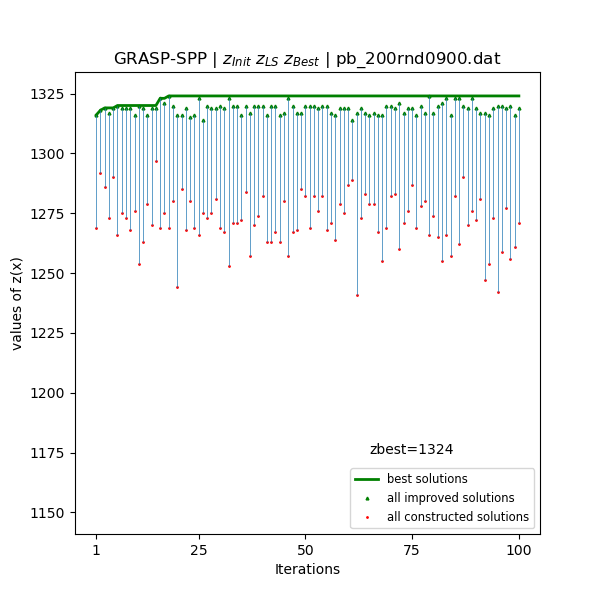
\includegraphics[height=8cm]{Traceofarun.png}}
    \vspace{5mm}
  
\end{frame}

%
%-----------------------------------------------------------
%
\begin{frame}
  \frametitle{References}
\vspace{3mm}

{\scriptsize
\begin{itemize}

\item 
Jeff Bezanson, Alan Edelman, Stefan Karpinski and Viral B. Shah.
Julia: A Fresh Approach to Numerical Computing. 
\textit{SIAM Review}, 59: 65--98. 2017.
\vspace{2mm}

\item 
 Miles Lubin, Oscar Dowson, Joaquim {Dias Garcia}, Joey Huchette, Beno{\^i}t Legat, Juan Pablo Vielma.
{JuMP} 1.0: {R}ecent improvements to a modeling language for mathematical optimization.
\textit{Mathematical Programming Computation}.
2023.
\vspace{2mm}

\item 
Thomas A. Féo and Mauricio G.C. Resende.  
A probabilistic heuristic for a computationally difficult set covering problem.
\textit{Operations  Research  Letters}, 8:67-71,1989.
\vspace{2mm}

\item 
Mauricio G.C. Resende and Celso C. Ribeiro.  
\textit{Optimization by GRASP: Greedy Randomized Adaptive Search Procedures.}
332 pages. Springer, 2018.
\vspace{2mm}

\item 
Xavier Delorme, Xavier Gandibleux, and Joaquin Rodriguez. 
GRASP for set packing problems.
 \textit{European Journal of Operational Research}, 153(3):564-580, 2004.
\vspace{2mm}

\end{itemize}
}
   
\end{frame}





\end{document}
% 
% -------------------------------------------------------------------------------------------------------------------------------------------------------
%

\begin{frame}
%  \frametitle{Slides suivants...}
  
      \vspace{7mm}
    \centerline{
\includegraphics[height=6cm]{imageMire.png}}
    \vspace{5mm}
    
%  \href{run:./FctOI-1-1-THEME1representations.pdf}{\centerline{\Large{\textcolor{nblue}{Next: Getting started}}}}
  
\end{frame}

  
\end{document}  



    


